\documentclass[10pt]{article}
\usepackage{icmlko}

\icmlmeta{IP 파운데이션 월드모델}{195}{보이지 않는 이득은 못 가져간다}{손잡이 둘을 같이 고르면 더 나빠진다. 하나씩 순차로 고르면 최적에 가까워지고, 규약이 2단계를 거절한다 --- 그 거절이 옳은지 유보 격자를 다 열어 봤다}

\begin{document}

\twocolumn[
\icmlheader

\begin{abstract}
노트 194가 최근 가중 $\tau$ 로 $+$0.0304 를 얻고 ``$\tau$ 와 $\alpha$ 를
같이 고르면''을 남겼다. \textbf{같이 고르면 더 나쁘다} --- 안쪽이
$(\tau{=}8, \alpha{=}100)$ 을 고르고 유보 $+$0.3880 인데, $\tau$ 만 고른
$+$0.4012 보다 \textbf{0.013 낮다.} 까닭이 보인다: 2차원이 되면 주변 곡선이
절반으로 뭉개진다 --- $\tau$ 1차원 훑기의 폭이 0.029(0.478$\sim$0.507)인데
2차원 주변 평균의 폭은 0.015 다. \textbf{그리고 규약이 그것을 막는다} ---
봉우리 0.354 · $\tau$ 주변 단조 0.200 · $\alpha$ 주변 단조 0.000 으로 셋 다
문턱 아래다. 그래서 \textbf{순차}로 했다: 1단계에서 $\alpha$ 를 고정하고
$\tau$ 를 1차원으로 고르고(통과 --- 단조 0.943, $\tau{=}2$), 2단계에서 그
$\tau$ 로 되뽑은 자료에서 $\alpha$ 를 1차원으로 고른다. \textbf{2단계가
막힌다} --- 봉우리 0.296 · 단조 0.000. 그래서 $\alpha$ 는 1 로 남고 결과가
$(\tau{=}2, \alpha{=}1)$ 의 $+$0.4012 다. \textbf{그 거절이 옳았나.} 유보
격자를 다 열어 봤다(정직하게 말하면 이건 확인이지 선택이 아니다).
\textbf{격자 최고는 $(\tau{=}1, \alpha{=}500)$ 의 $+$0.4084} 이고 순차는
$+$0.4012 다 --- \textbf{0.0072 를 남긴다.} 그리고 유보에서 $\alpha$ 는
\emph{모든} $\tau$ 에서 단조 증가한다. \textbf{2단계 거절은 방향이 틀린 게
아니라 안쪽에서 안 보인 것이다.} 되뽑기가 안쪽 학습을 더 작고 시끄럽게
만들어 $\alpha$ 신호를 지웠다. \textbf{그래서 이 노트의 결론은 값의
계산서다} --- 규약은 같이 고르기의 $-$0.0132 를 막고 대신 보이지 않는
$+$0.0072 를 놓친다. \textbf{순이득 $+$0.006 이고, 더 중요하게는 어느 쪽도
유보를 안 보고 정해진다.}
\end{abstract}
]

\begin{figure*}[t]
\centering
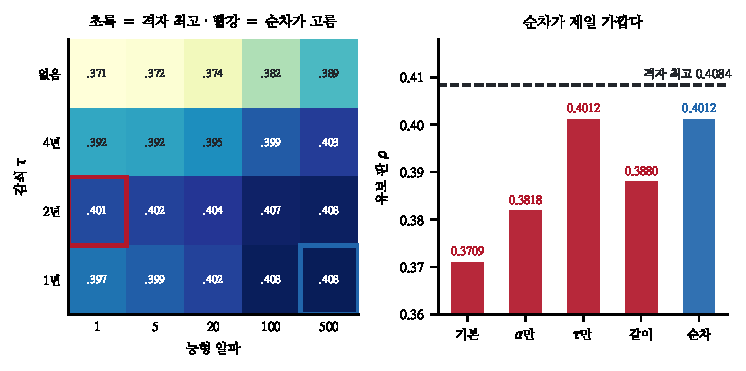
\includegraphics[width=.74\textwidth]{figs/seen.pdf}
\caption{왼쪽 --- 유보 격자. 초록이 최고, 빨강이 순차가 고른 곳.
오른쪽 --- 순차가 제일 가깝다.}
\end{figure*}

\section{같이 고르면 더 나쁘다}

\begin{table}[t]
\centering\tsize
\caption{F6 능형. 유보 판 $\rho$.}
\begin{tabular}{llr}
\toprule
절차 & 고른 것 & 판 \\
\midrule
기본 & $\tau$ 없음 · $\alpha{=}1$ & .3709 \\
$\alpha$ 만 & $\alpha{=}100$ & .3818 \\
\textbf{$\tau$ 만} & $\tau{=}2$ & \textbf{.4012} \\
\textbf{같이} & $\tau{=}8$ · $\alpha{=}100$ & \textbf{.3880} \\
\bottomrule
\end{tabular}
\end{table}

\claimx{\textbf{같이 고른 것이 $\tau$ 만 고른 것보다 0.013 낮다.} 손잡이를
하나 더 준 것이 손해다.}{2차원이 되면 주변 곡선이 뭉개진다 --- $\tau$ 1차원
훑기의 폭이 0.029 인데 2차원 주변 평균은 0.015 다. \textbf{다른 손잡이를
평균해 없애면 신호도 절반이 없어진다.}}

\claimx{\textbf{규약이 막는다} --- 봉우리 0.354 · $\tau$ 주변 단조 0.200 ·
$\alpha$ 주변 단조 0.000. 셋 다 문턱 아래다.}{노트 194에서 단조 지수를
1차원에만 쓰기로 한 것이 여기서 값을 한다 --- 2차원에서는 주변 단조를
계산할 수 있지만 그것도 뭉개져서 안 선다.}

\section{순차로 하면 가까워진다}

\begin{table}[t]
\centering\tsize
\caption{한 번에 하나씩.}
\begin{tabular}{llrrl}
\toprule
& 고름 & 봉우리 & 단조 & \\
\midrule
1단계 $\tau$ & \textbf{2년} & .298 & \textbf{.943} & \textbf{통과} \\
2단계 $\alpha$ & (100) & .296 & \textbf{.000} & \textbf{막힘} \\
\midrule
결과 & $\tau{=}2$ · $\alpha{=}1$ & & & \textbf{.4012} \\
\bottomrule
\end{tabular}
\end{table}

\claimx{\textbf{2단계가 막힌다.} 되뽑은 자료에서 $\alpha$ 안쪽 곡선이 봉우리도
단조도 아니다.}{되뽑기가 안쪽 학습을 더 작고 시끄럽게 만든다 --- 같은 행 수를
뽑지만 중복이 생겨 \emph{서로 다른} 행이 줄어든다. \textbf{$\alpha$ 를 보는
눈이 흐려진 것이다.}}

\section{거절이 옳았나}

\begin{table}[t]
\centering\tsize
\caption{유보 격자 전체. \emph{확인용이지 선택용이 아니다.}}
\begin{tabular}{lrrrrr}
\toprule
$\tau$ & $\alpha1$ & $5$ & $20$ & $100$ & $500$ \\
\midrule
없음 & .3709 & .3716 & .3744 & .3818 & .3888 \\
4년 & .3915 & .3921 & .3945 & .3992 & .4028 \\
\textbf{2년} & \textbf{.4012} & .4021 & .4035 & .4072 & .4076 \\
1년 & .3971 & .3989 & .4020 & .4081 & \textbf{.4084} \\
\bottomrule
\end{tabular}
\end{table}

\claimx{\textbf{$\alpha$ 는 모든 $\tau$ 에서 단조 증가한다.} 유보에서는
$\alpha{=}500$ 이 늘 제일 낫다 --- \textbf{2단계 거절은 방향이 틀린 게
아니다.}}{그러니 이건 ``규약이 잘못 막았다''가 아니라 \textbf{``안쪽에서
안 보이는 것을 못 가져간다''} 다. 노트 179의 ``틀린 값은 이미 죽어
있었다''와 성질이 다르다 --- 거기서는 진짜로 없었고 여기서는 있는데 안
보인다.}

\claimx{\textbf{값의 계산서.} 규약은 같이 고르기의 $-$0.0132 를 막고 보이지
않는 $+$0.0072 를 놓친다 --- 순이득 $+$0.0060.}{그리고 더 중요한 것은
\textbf{어느 쪽도 유보를 안 보고 정해진다}는 것이다. 이 표를 연 것은
사후 확인이고, 이 표를 보고 $(\tau{=}1, \alpha{=}500)$ 을 채택하면 노트
126이 잡은 그 잘못이다.}

\claimx{\textbf{채택은 순차 결과다} --- \texttt{F6\_directpool\_recent} 가
$+$0.4004 로 이미 등록돼 있고, 여기서 확인한 것은 그 위에 $\alpha$ 를
얹으면 안 된다는 것이다.}{챔피언은 여전히 F18 배깅($+$0.4490)이다 ---
\textbf{능형이 $+$0.3709 에서 $+$0.4012 로 올라 격차가 0.078 에서 0.048 로
줄었다.}}

\begin{table}[t]
\centering\tsize
\caption{남은 것.}
\begin{tabular}{ll}
\toprule
\textbf{되뽑기} & 가중을 직접 주면 안쪽이 안 흐려질 것 \\
F18 & $\tau{=}2$ 가 유보에서 $+$0.0117 인데 못 가져간다 \\
순서 & $\alpha$ 를 먼저 고르면 달라지나 \\
\bottomrule
\end{tabular}
\end{table}

첫 줄이 두 문제를 한 번에 풀 수 있다. 지금은 되뽑기로 가중을 흉내 내는데,
그것이 안쪽 학습의 \emph{서로 다른} 행 수를 줄여 $\alpha$ 신호를 지운다.
\texttt{sample\_weight} 로 직접 주면 행이 안 줄고 안쪽이 안 흐려진다 ---
\textbf{그러면 2단계가 통과할 수 있고 $+$0.007 을 되찾는다.} 다만 정식화마다
가중을 받는 자리가 달라 하네스를 손봐야 한다. \textbf{그게 다음이다.}

\end{document}
